%%%%%%%%%%%%%%%%%%%%%%%%%%%%%%%%%%%%%%%%%%%%%%%%%%%%%%%%%%%%%%%%%%%%%%%%%%%%%%%%
%2345678901234567890123456789012345678901234567890123456789012345678901234567890
%        1         2         3         4         5         6         7         8

\documentclass[letterpaper, 10 pt, conference]{ieeeconf}  % Comment this line out if you need a4paper

%\documentclass[a4paper, 10pt, conference]{ieeeconf}      % Use this line for a4 paper

\IEEEoverridecommandlockouts                              % This command is only needed if 
                                                          % you want to use the \thanks command

\overrideIEEEmargins                                      % Needed to meet printer requirements.
\usepackage{graphicx}
\usepackage{amsmath}
\usepackage{animate}


%In case you encounter the following error:
%Error 1010 The PDF file may be corrupt (unable to open PDF file) OR
%Error 1000 An error occurred while parsing a contents stream. Unable to analyze the PDF file.
%This is a known problem with pdfLaTeX conversion filter. The file cannot be opened with acrobat reader
%Please use one of the alternatives below to circumvent this error by uncommenting one or the other
%\pdfobjcompresslevel=0
%\pdfminorversion=4

% See the \addtolength command later in the file to balance the column lengths
% on the last page of the document

% The following packages can be found on http:\\www.ctan.org
%\usepackage{graphics} % for pdf, bitmapped graphics files
%\usepackage{epsfig} % for postscript graphics files
%\usepackage{mathptmx} % assumes new font selection scheme installed
%\usepackage{times} % assumes new font selection scheme installed
%\usepackage{amsmath} % assumes amsmath package installed
%\usepackage{amssymb}  % assumes amsmath package installed

\title{\LARGE \bf
Eye and Gaze Tracking in Real-Time Using Dlib's Face Recognition Library
}


\author{Somesh Bagadiya}



\begin{document}



\maketitle
\thispagestyle{empty}
\pagestyle{empty}


%%%%%%%%%%%%%%%%%%%%%%%%%%%%%%%%%%%%%%%%%%%%%%%%%%%%%%%%%%%%%%%%%%%%%%%%%%%%%%%%
\begin{abstract}

This report presents an in-depth exploration into the realm of eye tracking and gaze analysis utilizing the capabilities of Dlib's Face Recognition library. The project aims to leverage facial landmark detection provided by Dlib to implement robust eye tracking mechanisms and accurately estimate gaze direction. By extracting detailed information from facial landmarks, the system tracks eye movements in real-time, offering applications in fields such as human-computer interaction, assistive technologies, and virtual reality environments.

The report outlines the methodology employed for facial landmark detection, focusing on Dlib's Face Recognition library and its suitability for eye and gaze tracking applications. Emphasis is placed on the challenges encountered and the strategies employed to enhance accuracy and efficiency in real-time scenarios. Additionally, the study investigates the limitations of the implemented system and discusses potential avenues for future enhancements..

\end{abstract}


%%%%%%%%%%%%%%%%%%%%%%%%%%%%%%%%%%%%%%%%%%%%%%%%%%%%%%%%%%%%%%%%%%%%%%%%%%%%%%%%
\section{INTRODUCTION}

In the ever-evolving landscape of human-computer interaction, the integration of eye tracking technologies has emerged as a transformative force. At the core of this evolution lies a fundamental question: Why utilize the eyes as a means of providing input to computers? This inquiry forms the cornerstone of our exploration into the implementation of real-time eye tracking and gaze analysis, specifically leveraging the capabilities of Dlib's Face Recognition library.

The advantages of employing eyes as a source of input are manifold. From a practical standpoint, the eyes offer a natural and intuitive means of communication with computing systems. Their versatility allows users to seamlessly interact with devices without the need for physical interfaces, offering a level of convenience and efficiency that transcends traditional input methods. However, amidst the advantages lie challenges. What are the disadvantages of eye tracking? Unraveling these complexities is crucial in understanding the nuanced dynamics of this technology.

As we navigate through the project, we will not only delve into the theoretical underpinnings but also scrutinize its real-world applications. From enhancing user experiences in day-to-day interactions to addressing critical issues like drowsiness detection and real-time attention monitoring, eye tracking demonstrates its potential to transcend mere convenience and delve into the realm of safety and well-being.

Delving deeper, we will scrutinize the distinction between eye tracking and gaze tracking. What sets these two apart, and why does it matter? The nuanced differences play a crucial role in unlocking specific applications, such as precise mouse control and dynamic heat mapping. Through this exploration, we aim to unravel the intricacies of eye and gaze tracking, offering a comprehensive understanding of their potential and limitations in the broader landscape of human-computer interaction.


\section{Background and Motivation}

In the ever-expanding landscape of technological innovation, the quest for more intuitive and seamless ways of interacting with our digital environment has led to a reevaluation of conventional input methods. The advent of technologies like Augmented Reality (AR) and Virtual Reality (VR) has propelled the significance of eye tracking to the forefront. Despite conventional input methods, why consider the eyes as a primary source of input? The answer lies in the unparalleled potential of the eyes to serve as a direct interface between the user and technology, particularly in AR and VR environments where hands-free operation is pivotal.

Our eyes, as the primary means through which we perceive and interact with the world, naturally lend themselves to becoming a fundamental input source. Why is this natural, and what advantages does it offer? Eyes, being our primary tools for environmental interaction, provide a seamless and instinctive way to engage with technology. By leveraging eye movements as a primary input, users can transcend the constraints of physical touch, traditional mouse, or keyboard inputs. This not only aligns with the evolving landscape of hands-free technology but also introduces a paradigm shift where the latency between thought and implementation is significantly reduced.

Operating on the principle of simply looking at an object to execute a command, eye tracking not only enhances the convenience of interaction but also introduces a transformative level of speed and efficiency. This immediacy in command execution can prove invaluable in various contexts, from enhancing user experiences to optimizing efficiency in professional and personal computing. Furthermore, eye tracking can seamlessly complement existing input methods, acting as an assistive input that augments convenience and speed.

As we delve into the implementation of real-time eye tracking using Dlib's Face Recognition library, these motivations underscore the inherent potential of eyes as a central input source. The exploration of this technology aligns with the broader goal of not only advancing human-computer interaction but also redefining the way we engage with and command our digital environments.


\section{Advantages and Disadvantages of Eye Tracking}

In the pursuit of revolutionizing human-computer interaction, eye tracking technology emerges as a powerful tool with a host of advantages. Simultaneously, it is essential to acknowledge the challenges and disadvantages that accompany this innovative approach.

\subsection{Advantages}

\begin{enumerate}
    \item \textbf{Natural Interaction:} Eyes serve as our primary means of perceiving and interacting with the world. Leveraging eye movements as an input method aligns seamlessly with our natural behaviors, making it an intuitive and user-friendly interaction paradigm.
    
    \item \textbf{Hands-Free Operation:} One of the most significant advantages of eye tracking is its potential for hands-free operation. In scenarios where physical touch or traditional input devices are impractical, eyes can serve as a direct and efficient interface, particularly in augmented and virtual reality environments.
    
    \item \textbf{Reduced Latency:} Eye tracking minimizes the latency between thought and action. Users can execute commands by simply looking at an object or point of interest, significantly enhancing the immediacy and speed of interactions.
    
    \item \textbf{Assistive Input:} Eye tracking can act as an assistive input method, complementing traditional inputs and offering an additional layer of convenience. This feature is particularly valuable for individuals with motor impairments, providing an alternative means of interacting with technology.
    
    \item \textbf{Enhanced User Experiences:} By tracking gaze and eye movements, applications can adapt and respond to user behavior in real-time, leading to personalized and enhanced user experiences. This is especially relevant in gaming, immersive storytelling, and other entertainment applications.
\end{enumerate}

\subsection{Disadvantages}

\begin{enumerate}
    \item \textbf{Calibration Challenges:} Achieving accurate eye tracking may require calibration, a process that introduces complexity and potential user inconvenience. Calibration becomes critical for precise gaze estimation, particularly in scenarios where accuracy is paramount.
    
    \item \textbf{Cost of Implementation:} High-quality eye-tracking hardware and software can be relatively expensive, limiting widespread adoption. The cost factor presents a challenge in making eye tracking technology accessible to a broader audience.
    
    \item \textbf{Privacy Concerns:} Eye tracking involves the collection of sensitive biometric data. Privacy concerns may arise regarding the storage and use of this data, necessitating robust security measures to safeguard user information.
    
    \item \textbf{Environmental Limitations:} Variations in lighting conditions, the presence of eyeglasses, or other environmental factors can impact the accuracy of eye tracking. Overcoming these challenges requires sophisticated algorithms and hardware.
    
    \item \textbf{User Fatigue:} Extended use of eye tracking may lead to user fatigue or discomfort. Prolonged periods of intense focus on a screen or device may strain the eyes, necessitating ergonomic considerations and periodic breaks.
\end{enumerate}

As we navigate the implementation of real-time eye tracking using Dlib's \texttt{face\_recognition} library, these advantages and disadvantages form crucial considerations. Balancing the inherent strengths with the challenges is essential to harness the full potential of eye tracking technology in diverse applications.


\section{Eye Tracking vs. Gaze Tracking Technology}

In the realm of human-computer interaction, distinguishing between eye tracking and gaze tracking is crucial, as each technology serves distinct purposes and applications. While these terms are often used interchangeably, they refer to different aspects of monitoring eye behavior.

\subsection{Eye Tracking}

\textit{Eye tracking technology} primarily focuses on tracing the movement of the eyes as a whole. It involves capturing the broader spectrum of eye movements, including saccades (rapid shifts in gaze), fixations (steady gaze on a point), and smooth pursuits (tracking a moving object). The goal is to comprehend how eyes explore and navigate the visual environment, providing insights into visual attention and cognitive processes.

\subsubsection{Advantages of Eye Tracking:}
\begin{itemize}
    \item \textbf{Comprehensive Analysis:} Eye tracking offers a comprehensive analysis of overall eye movements, enabling a holistic understanding of user engagement and attention.
    
    \item \textbf{Behavioral Insights:} It provides behavioral insights, helping researchers and designers assess user reactions to visual stimuli and interface elements.
\end{itemize}

\subsubsection{Disadvantages of Eye Tracking:}
\begin{itemize}
    \item \textbf{Limited Precision:} While suitable for broad gaze patterns, eye tracking may lack the precision required for specific point-of-gaze applications.
    
    \item \textbf{Calibration Requirements:} Calibration is often necessary to ensure accurate tracking, adding a layer of complexity.
\end{itemize}

\subsection{Gaze Tracking}

\textit{Gaze tracking}, on the other hand, zeroes in on the specific point where the eyes are focused, commonly referred to as the point of gaze. This technology is more concerned with pinpointing the exact location in the user's field of view where visual attention is concentrated. Gaze tracking is crucial for applications demanding precise interaction, such as controlling a cursor or selecting objects.

\subsubsection{Advantages of Gaze Tracking:}
\begin{itemize}
    \item \textbf{High Precision:} Gaze tracking offers high precision, allowing for accurate determination of the user's focal point.
    
    \item \textbf{Point-of-Gaze Interaction:} It facilitates point-of-gaze interaction, enabling users to control devices or interfaces with remarkable accuracy.
\end{itemize}

\subsubsection{Disadvantages of Gaze Tracking:}
\begin{itemize}
    \item \textbf{Limited Contextual Insights:} Gaze tracking may provide less contextual information about broader eye movements and visual exploration.
    
    \item \textbf{Challenges in Dynamic Environments:} Variations in lighting, user position, or external factors can pose challenges to maintaining accurate gaze tracking.
\end{itemize}


While eye tracking and gaze tracking technologies share the common goal of understanding visual behavior, their scopes and applications differ. Eye tracking provides a holistic view of eye movements, suitable for behavioral analysis, while gaze tracking excels in precision applications requiring knowledge of the exact point where the user is looking. In our exploration of real-time eye tracking using Dlib's \texttt{face\_recognition} library, understanding these distinctions is paramount for effectively applying the technology to diverse use cases.

\section{Eye Tracking Application: Drowsiness Detection}

\subsection{Introduction}

Drowsiness detection plays a pivotal role in ensuring the safety of individuals, especially in contexts such as driving or operating heavy machinery. In this section, we delve into the implementation of a drowsiness detection system using eye tracking technology. The goal is to leverage eye movement patterns to identify signs of drowsiness and prompt timely interventions.

\subsection{Methodology}

Our drowsiness detection system relies on the analysis of key eye movement metrics, such as blink frequency and duration of eye closures. The assumption is that as an individual becomes drowsy, there is a tendency for changes in these metrics. A threshold-based approach is adopted, where deviations from normal eye movement patterns trigger an alert.

\subsection{Implementation}

The implementation of drowsiness detection using eye tracking involves a series of steps to accurately monitor the driver's state based on eye movements. Here are the key steps undertaken in this process:

\begin{enumerate}
    \item \textbf{Face Detection:} Utilizing the Face Recognition Library, the system detects and locates the driver's face within the captured frame. This library returns essential facial landmarks, including the eyes, ears, mouth, and other distinctive features.
    
    \item \textbf{Eye Landmark Extraction:} After obtaining facial landmarks, specific points related to the eyes are extracted. These include the corners of the eyes, the top and bottom of each eye, as well as additional points on the top and bottom eyelids.

    \item \textbf{Eye Aspect Ratio (EAR) Calculation:} The Eye Aspect Ratio (EAR) is computed using the extracted eye features. The EAR is calculated using the formula:
    
    \[
    \text{EAR} = \frac{{\|B - D\| + \|E - F\|}}{{2 \|A - C\|}}
    \]

    Where:
    \begin{align*}
    A & : \text{Inner corner of the eye (leftmost point)} \\
    B & : \text{Top of the eye} \\
    C & : \text{Outer corner of the eye (rightmost point)} \\
    D & : \text{Bottom of the eye} \\
    E & : \text{Additional point on the top eyelid} \\
    F & : \text{Additional point on the bottom eyelid}
    \end{align*}

    This formula provides a quantitative measure of the eyes' openness.

    \item \textbf{Interpreting EAR for Drowsiness Detection:} The EAR provides valuable insights into the state of the driver's eyes. When the eyes are open, the EAR is relatively high. Conversely, when the eyes are closing or closed, the EAR decreases. Blinking typically involves a significant drop in EAR.

    \item \textbf{Threshold Comparison:} The calculated EAR is compared with a predefined threshold, often set around 0.2. If the EAR falls below this threshold, it indicates that the eyes are closing, signaling a potential state of drowsiness or inattention.

    \item \textbf{Alert Mechanism:} Upon detecting a decrease in EAR, signifying closed eyes, an alert mechanism is activated. A timer of approximately 3 seconds is initiated to determine if the eyes remain closed during this period. If so, an alert is triggered, often in the form of a beep sound, indicating that the driver may be drowsy or not fully attentive.

    \item \textbf{Timer Reset:} Once the eyes are open again, the timer is reset, ensuring that the system is ready to detect subsequent instances of drowsiness.

\end{enumerate}

This systematic approach to drowsiness detection demonstrates the effectiveness of utilizing eye tracking technology for real-time monitoring and alerting in critical scenarios, such as driving.

\subsection{Results}

The drowsiness detection system demonstrates promising results in identifying instances of drowsiness based on eye movement patterns. Through real-time monitoring, the system can promptly alert the user or relevant stakeholders, mitigating potential risks associated with drowsy states.

\begin{figure}
  \centering
  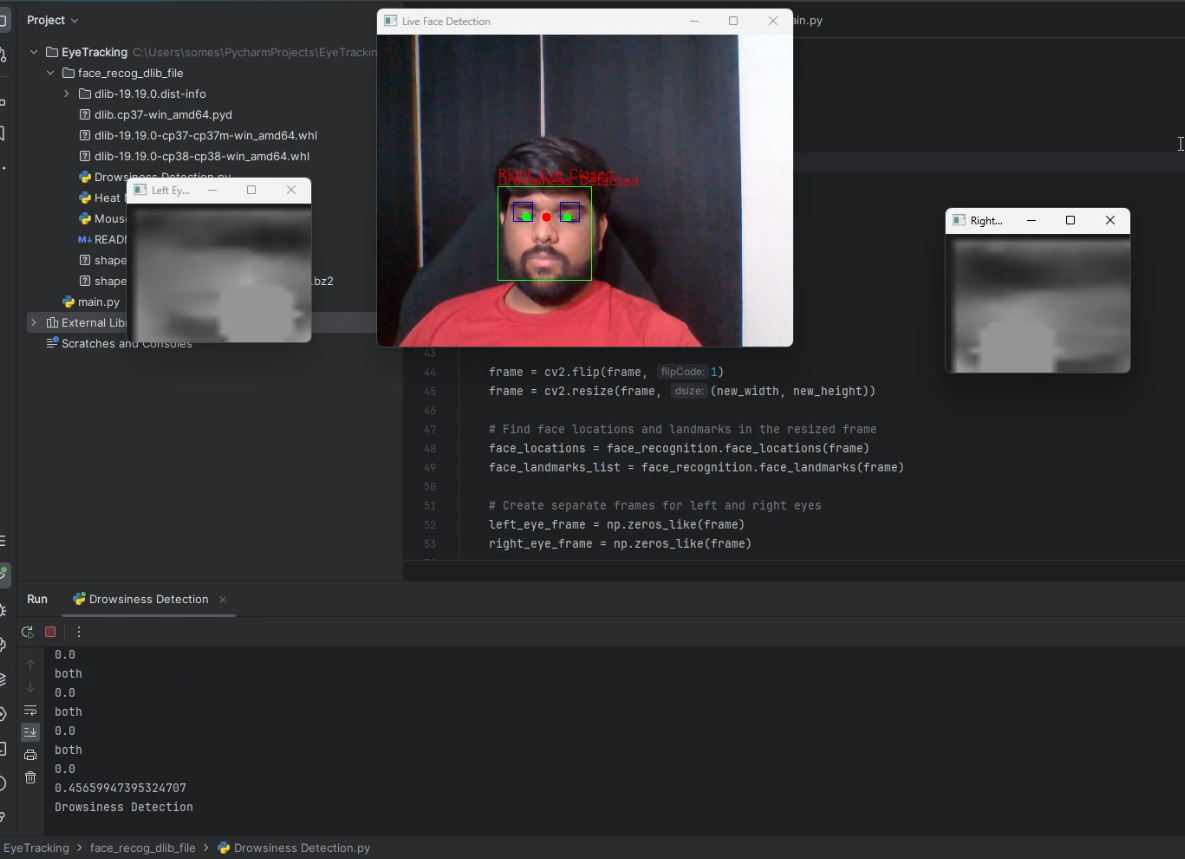
\includegraphics[width=0.45\textwidth]{Drowsiness1.png} % Replace "image_filename" with the actual filename of your image
  \caption{Image shows a output frame depecting the software has detected drowsiness }
  \label{fig:your_label}
\end{figure}

\subsection{Challenges and Future Improvements}

While the current implementation shows encouraging results, challenges such as variations in lighting conditions and individual differences pose ongoing considerations. Future improvements could involve incorporating machine learning techniques to adapt to individual patterns and refining the system's sensitivity to environmental factors.

\section{Eye Tracking Application: Mouse Control}

\subsection{Introduction}

In this section, we delve into the specific implementation of mouse control using eye tracking technology. The goal is to enable users to interact with the computer by intuitively moving the mouse cursor with their eyes. This hands-free approach enhances accessibility and provides an alternative input method for individuals with motor impairments.

\subsection{Methodology}

The methodology involves leveraging eye movements to control the mouse cursor. By accurately tracking the direction of the eye movement, the system translates this information into mouse cursor movements on the screen. This approach allows for a natural and responsive interaction without the need for traditional input devices.

\subsection{Implementation}

The implementation of mouse control using eye tracking involves the following steps:

\begin{enumerate}
    \item \textbf{Face Detection:} Leveraging the Face Recognition Library, the system detects the user's face and obtains facial landmarks, including the eyes, ears, mouth, and other distinctive features.
    
    \item \textbf{Eye Landmark Extraction:} Extracting specific points related to the eyes from the obtained facial landmarks. These points include the corners of the eyes, the top and bottom of each eye, as well as additional points on the top and bottom eyelids.
    
\item \textbf{Eye Center Calculation:} The midpoint of the eyes is calculated using the following equations:

The center of each eye is determined by computing the mean of all the eye landmarks obtained from facial recognition. The mean is calculated separately for the x and y coordinates of the center of the eye:

\begin{equation}
\text{{left\_eye\_centX}} = \frac{{\sum_{{i \in \text{{left\_eye\_landmarks}}}} i[0]}}{{\text{{len}}(\text{{left\_eye\_landmarks}})}}
\end{equation}

\begin{equation}
\text{{left\_eye\_centY}} = \frac{{\sum_{{i \in \text{{left\_eye\_landmarks}}}} i[1]}}{{\text{{len}}(\text{{left\_eye\_landmarks}})}}
\end{equation}

A similar calculation is applied for the right eye. The resulting \text{{left\_eye\_centX}}, \text{{left\_eye\_centY}}, \text{{right\_eye\_centX}}, and \text{{right\_eye\_centY}} are essential for tracking the movement of each eye during mouse control.

\begin{equation}
\text{{eye\_midX}} = \frac{{\text{{left\_eye\_centX}} + \text{{right\_eye\_centX}}}}{2}
\end{equation}

\begin{equation}
\text{{eye\_midY}} = \frac{{\text{{left\_eye\_centY}} + \text{{right\_eye\_centY}}}}{2}
\end{equation}

These equations compute the average x and y coordinates of the center of each eye and the midpoint between the eyes, respectively. The \text{{eyes\_midpoint}} is a crucial parameter for tracking the movement of the eyes during mouse control.

    \item \textbf{Mouse Movement:} As the user moves their eyes, the system continuously calculates the center of the eyes and adjusts the mouse cursor's position on the screen accordingly. This is achieved using the PyAutoGUI library to control the mouse.

    \item \textbf{Blink Detection for Clicking:} Utilizing left eye blinks as a mechanism for mouse clicks. The same logic used in drowsiness detection for blink detection is applied, but with a modified EAR threshold set to 0.25. When a blink is detected, it is interpreted as a click action.

\end{enumerate}

This implementation showcases the integration of eye tracking technology to control the mouse cursor, providing an alternative hands-free input method. The combination of eye movement tracking and blink detection enhances the system's functionality, allowing users to interact with their computers using eye gestures.



\subsection{Results}

The mouse control system demonstrates effective and responsive cursor movements based on the user's eye gaze. Users can navigate the cursor across the screen by simply looking at the desired location, offering a hands-free alternative that can be particularly beneficial for those with motor disabilities or in scenarios where traditional input devices are challenging to use.

\begin{figure}
  \centering
  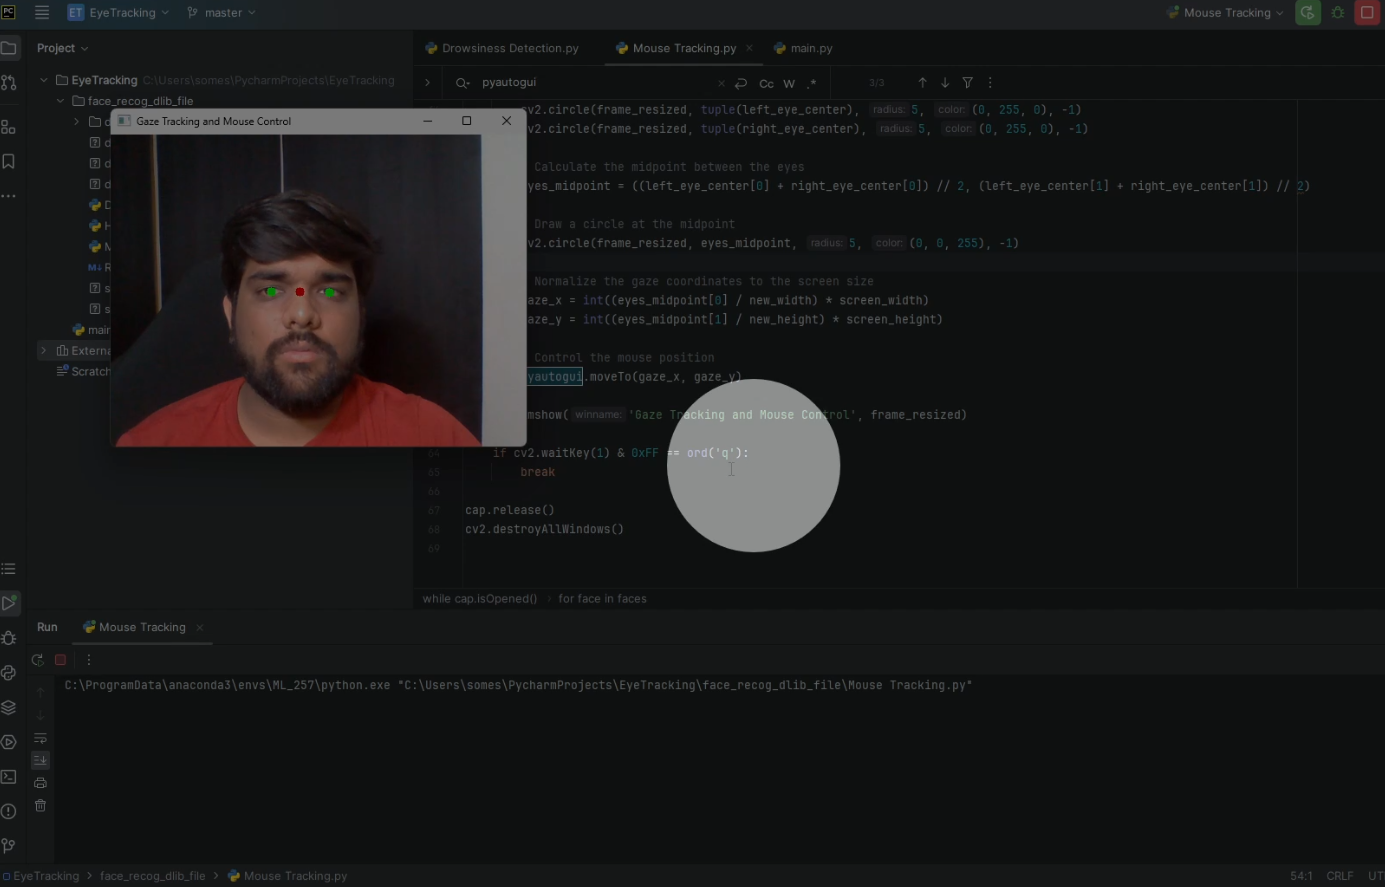
\includegraphics[width=0.45\textwidth]{Mouse1.png} % Replace "image_filename" with the actual filename of your image
  \caption{Image shows a output frame }
  \label{fig:your_label}
\end{figure}


\subsection{Challenges and Future Improvements}

Challenges in mouse control implementation revolve around calibration accuracy and ensuring consistent performance across various user scenarios. Future improvements may involve refining calibration algorithms, exploring machine learning models for personalized calibration, and addressing environmental factors that could impact tracking accuracy.



\section{Gaze Tracking Application: Heat Mapping}

\subsection{Introduction}

Gaze tracking opens up avenues for understanding user attention and interaction patterns. In this section, we explore the implementation of a gaze tracking application focused on generating heat maps based on the user's point of gaze. This technology provides valuable insights into areas of interest and can be applied in various fields, from usability studies to user experience optimization.

\subsection{Methodology}

The gaze tracking system captures and records the user's point of gaze in real-time. The methodology involves analyzing eye movements, specifically focusing on the direction and duration of gaze. By mapping these points onto the screen, a heat map is generated, visually representing the regions that attract the most attention.

\subsection{Implementation}

The implementation of the gaze tracking application involves the following steps:

\begin{enumerate}
    \item Utilizing the Face Recognition Library, the face is detected, and facial landmarks, including eyes, ears, and mouth, are obtained.
    \item Extracting eye features from the facial landmarks, including the corners of the eyes, top and bottom of the eye, and additional points on the top and bottom eyelids.
    \item Applying the Hough Circle function to extract circular objects from the frame, specifically targeting the pupils. The center of the detected circles represents the position of the pupils.
    \item Scaling the relative position of the pupils obtained from the frame to the display resolution.
    \item Gathering and storing the pupil positions in a list for later visualization.
    \item Plotting the collected points using Matplotlib to generate a heat map, providing a visual representation of the gaze tracking data.
\end{enumerate}

The resulting heat map is a valuable visualization that illustrates the points where the user's gaze was concentrated during the tracking process.

\subsection{Results}

The heat mapping application provides valuable insights into user attention patterns. The generated heat maps offer a visual representation of where users focus their gaze during interaction with a screen or interface. This information is crucial for optimizing design elements and improving overall user experience.

\begin{figure}
  \centering
  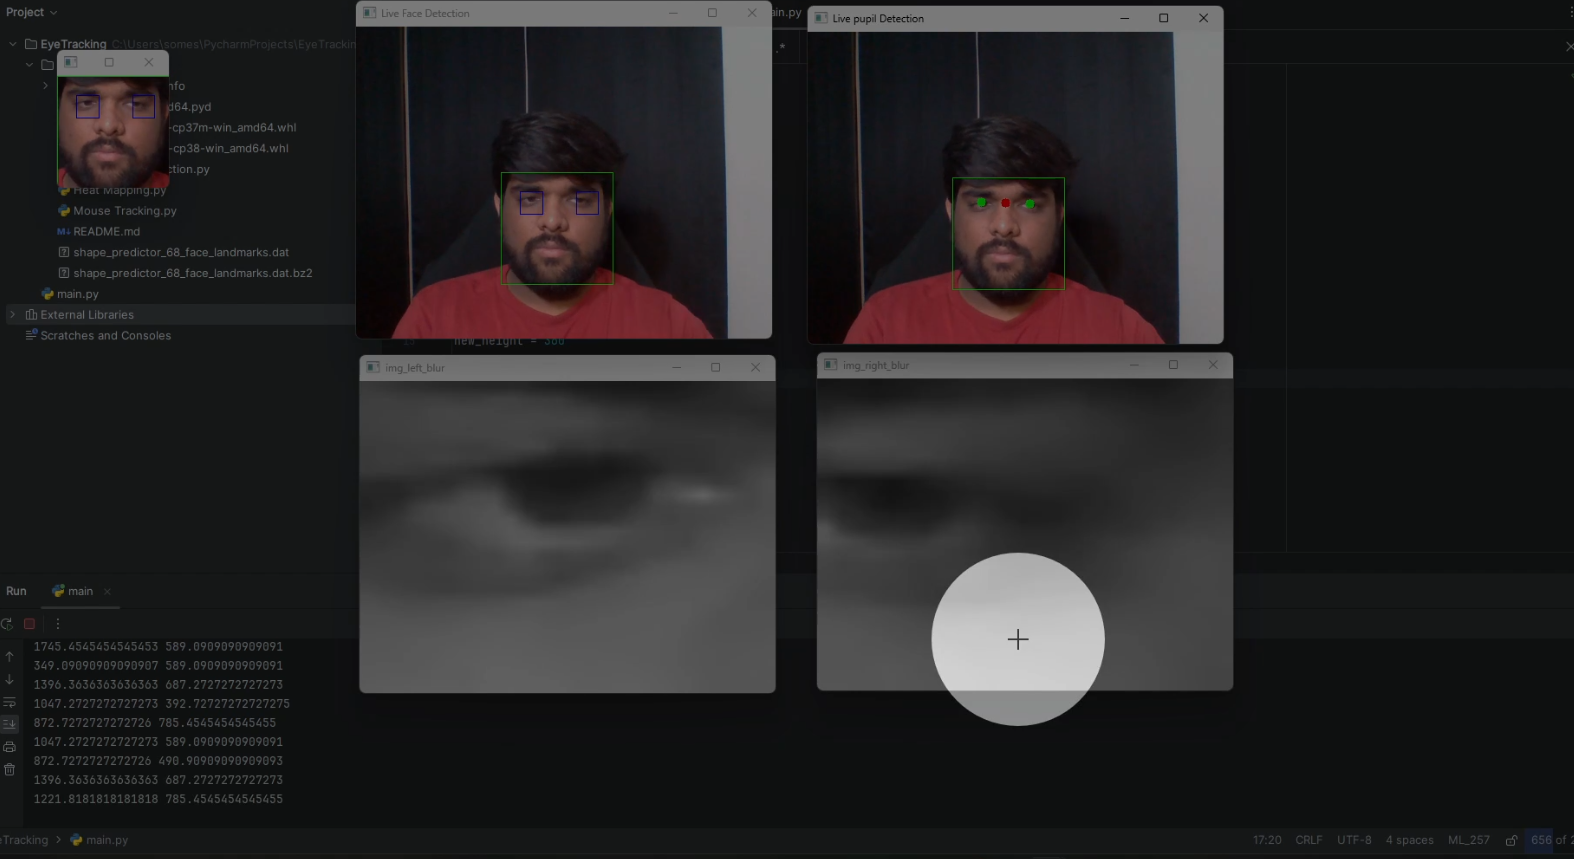
\includegraphics[width=0.45\textwidth]{heat1.png} % Replace "image_filename" with the actual filename of your image
  \caption{Image shows a output frame }
  \label{fig:your_label}
\end{figure}

\begin{figure}
  \centering
  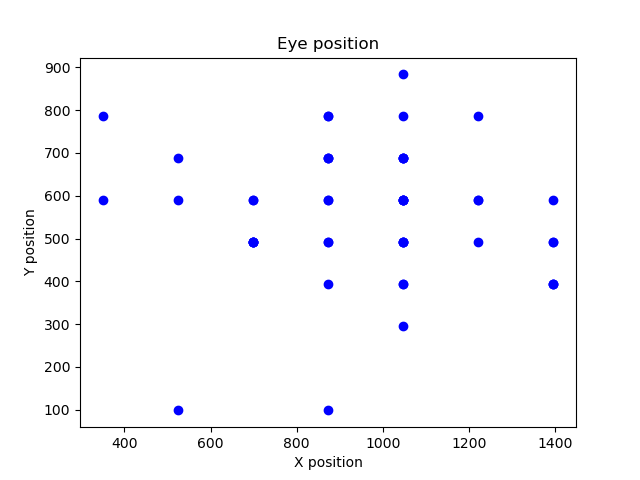
\includegraphics[width=0.45\textwidth]{heat2.png} % Replace "image_filename" with the actual filename of your image
  \caption{Image shows the final heat map output of the code }
  \label{fig:your_label}
\end{figure}

\subsubsection{Applications}

The generated heat maps find applications in:
\begin{itemize}
    \item Usability Studies: Understanding how users interact with websites, applications, or digital content.
    \item Marketing Research: Analyzing visual attention in advertisements and promotional materials.
    \item User Interface (UI) Optimization: Enhancing the placement of elements to capture user attention effectively.
\end{itemize}
\subsection{Challenges and Future Improvements}

While implementing the gaze tracking application, several challenges were encountered, and areas for potential improvement were identified. One major concern is the calibration of the system to achieve precise gaze tracking. Calibration plays a crucial role in accurately mapping the user's eye movements to the screen coordinates. Ensuring precise calibration is essential for the reliability of the generated heat map.

Future improvements could involve refining the calibration process to enhance accuracy and robustness. Additionally, exploring advanced gaze tracking algorithms and techniques may contribute to overcoming the challenges associated with different eye movements and user variations. Improving the overall tracking performance and addressing calibration issues would significantly enhance the effectiveness of the gaze tracking application.


\section{Conclusion}

\subsection{Key Findings}
This report has comprehensively explored the nuanced facets of eye and gaze tracking technologies, elucidating their significant potential and limitations. A pivotal finding of our study is the successful utilization of a standard webcam for eye detection, demonstrating that advanced eye tracking applications can be made accessible with minimal hardware requirements. Crucially, our implementations did not employ any calibration techniques, which, while simplifying the setup, also impacted the accuracy of the system. This highlights a trade-off between ease of use and precision in eye tracking technology. While eye tracking offers robust applications in areas like drowsiness detection and mouse control, its effectiveness, as we've shown, is achievable with basic webcams. However, its precision and user adaptability are contingent on algorithmic efficiency and environmental factors. Gaze tracking, particularly in heat mapping applications, provides invaluable insights into user engagement and behavior, though it faces challenges in accuracy under varied conditions.

\subsection{Contributions and Future Directions}
Our study contributes to the burgeoning field of eye and gaze tracking by providing a detailed comparative analysis of these technologies, alongside practical applications. The methodologies and implementations detailed in this report, especially the absence of calibration techniques, can serve as a foundation for future research. This approach demonstrates the potential for enhancing safety and accessibility in computing while also indicating areas for improvement in precision and reliability.

Looking forward, addressing the limitations of accuracy without calibration will be crucial. Developing more sophisticated algorithms and exploring alternative, non-invasive calibration methods could significantly enhance the practicality and effectiveness of eye and gaze tracking technologies. Moreover, the integration of these technologies in diverse fields such as virtual reality, healthcare, and automotive safety opens new avenues for innovation.

\subsection{Implications for Technology}
The implications of our findings extend beyond the immediate realm of eye and gaze tracking. They underscore the importance of user-centric design in technology development, emphasizing the need for technologies that are not only advanced but also intuitive and accessible. As we venture into an era increasingly dominated by AI and machine learning, the principles highlighted in this report will be crucial in guiding ethical and effective technological development.

\subsection{Conclusion Reflection}
In reflecting on our journey through this report, it is evident that eye and gaze tracking technologies are more than mere tools – they are gateways to understanding human-machine interaction on a deeper level. As we continue to push the boundaries of what is possible, it remains our collective responsibility to ensure that these technologies are developed responsibly, with a keen eye on their societal impact and ethical use.





\addtolength{\textheight}{-12cm}   % This command serves to balance the column lengths
                                  % on the last page of the document manually. It shortens
                                  % the textheight of the last page by a suitable amount.
                                  % This command does not take effect until the next page
                                  % so it should come on the page before the last. Make
                                  % sure that you do not shorten the textheight too much.

%%%%%%%%%%%%%%%%%%%%%%%%%%%%%%%%%%%%%%%%%%%%%%%%%%%%%%%%%%%%%%%%%%%%%%%%%%%%%%%%



%%%%%%%%%%%%%%%%%%%%%%%%%%%%%%%%%%%%%%%%%%%%%%%%%%%%%%%%%%%%%%%%%%%%%%%%%%%%%%%%



%%%%%%%%%%%%%%%%%%%%%%%%%%%%%%%%%%%%%%%%%%%%%%%%%%%%%%%%%%%%%%%%%%%%%%%%%%%%%%%%



%%%%%%%%%%%%%%%%%%%%%%%%%%%%%%%%%%%%%%%%%%%%%%%%%%%%%%%%%%%%%%%%%%%%%%%%%%%%%%%%


\begin{thebibliography}{99}

\bibitem {}  Dujuan Zhang; Jie Li; Zhenfang Shan, "Implementation of Dlib Deep Learning Face Recognition Technology
" in IEEE. Available: https://ieeexplore.ieee.org/document/9523885 [Accessed: 06 Sept 2021].

\bibitem {}  Primesh Pathirana, Shashimal Senarath, Dulani Meedeniya, Sampath Jayarathna, "Eye gaze estimation: A survey on deep learning-based approaches," ScienceDirect. Available: https://www.sciencedirect.com/science/article/abs/pii/S0957417422003347 [Accessed: 1 Aug 2022].

\bibitem {}  Sreeza Tarafder; Nasreen Badruddin; Norashikin Yahya; Ashvaany Egambaram "EEG-based Drowsiness Detection from Ocular Indices Using Ensemble Classification" in IEEE [Accessed: 28-30 May 2021]

\bibitem {} Anuradha Kar, Peter Corcoran "A Review and Analysis of Eye-Gaze Estimation Systems, Algorithms and Performance Evaluation Methods in Consumer Platforms" in ARIXV [Accessed: 5 Aug 2017]


\end{thebibliography}



\end{document}
 